\documentclass[10pt]{article}
\usepackage{fullpage}
\usepackage{graphicx}
\usepackage{amssymb}
\usepackage{qtree}
\newcommand{\tab}{\hspace*{2em}}
\newcommand{\tabb}{\hspace*{4em}}
\newcommand{\tabbb}{\hspace*{6em}}
\begin{document}
	\begin{flushright}
	Lindsey Bieda and Joe Frambach\\
	Dynamic Programming Problems\\
	9.26.2011
	\end{flushright}
	\noindent
	10.	The input for this problem consists of $n$ keys $K_1, \ldots, K_n$, with $K_1 < K_2 < \ldots , K_n$, and associated
			probabilities $p_1, \ldots, p_n$. The problem is to find the AVL tree for these keys that minimizes the expected
			depth of a key.  An AVL tree is a binary search tree with the property that every node has balance
			factor -1, 0, or 1. Give a polynomial time algorithm for this problem.\\
			\\
			% answer here
			The following code runs in polynomial time and uses a table based iterative approach in order to arrive at a solution.
			It requires that the array of of keys' probabilities are passed in. It initializes three main tables. The first
			is expected[] which holds the expected search costs for the trees which contain the keys from $K_i, \ldots, K_j$.
			The second, cost[], similarly holds the total expected cost for the trees which contain the keys from $K_i, \ldots, K_j$.
			Depth[] holds the maximum depth of the trees which contain the keys from $K_i, \ldots, K_j$. Root[] contains the index
			of the key that is the root of the AVL tree with keys $K_i, \ldots, K_j$ that has the lowest expected search cost.
			\begin{verbatim}
			provided p[] array of n key probabilities 
			 
			for i in (1,n+1):
			  expected[i,i-1] = 0
			  cost[i,i-1]     = 0
			  depth[i,i-1]    = 1
			  
			for l in (1,n):            // consider trees with l keys in them
			  for i in (1,n-l+1):      // consider trees starting with Ki 
			    j = i + l - 1          // and ending with Kj
			    expected[i,j] = infinity
			    cost[i,j] = cost[i,j-1] + p[j]
			    for r in (i,j):        // find the best root
			      expectedSum = expected[i, r-1] + expected[r+1, j] + cost[i,j]
			      if abs(depth[i,r-1], depth[r+1,j]) > 1:
			        \\ resulting tree would be unbalanced
			        expected[i,j] = infinity
			      if expectedSum < expected[i,j]:
			        expected[i,j] = expectedSum
			        root[i,j]     = r
			        depth[i,j]    = max(depth[i,r-1], depth[r+1,j]) + 1
			        
			  return expected, root
			\end{verbatim}
			
		\begin{figure}[h]
			\centering
				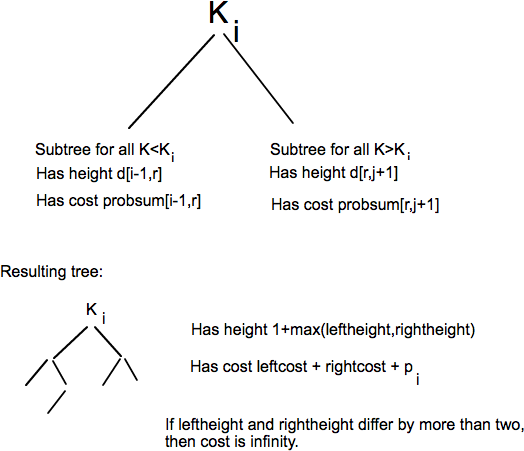
\includegraphics[width=300px]{dyn10.png}
			\label{fig:dyn10}
			\caption{showing the construction of $K_i, \ldots, K_j$ trees}
		\end{figure}
	\newpage
	.
	\newpage
	\noindent
	11.	The input consists of $n$ intervals over the real line. The output should be a collection $C$  of nonoverlapping 
			intervals such the sum of the lengths of the intervals in $C$ is maximized. Give a polynomial
			time algorithm for this problem.\\
			\\
			% answer here
\end{document}